% ===================================================================================
% Presentation: A Branch-and-Bound Method for Bilevel Parallel Machine Scheduling
%               with Adversarial Job Selection
% Author: Ole Damke, TU Braunschweig, April 2026
%
% Compile:  $env:TEXINPUTS="./tex//;"; xelatex -interaction=nonstopmode presentation.tex
% ===================================================================================
% !TEX program = xelatex-nobiber

\documentclass[fleqn,11pt,aspectratio=43]{beamer}
\usepackage[english]{babel}
\usetheme[blue,dark,colorblocks]{tubs}

% --- Fonts ---
\usepackage{fontspec}
\setmainfont{NexusSerifPro}[
  Path=./fonts/otf/, Extension=.otf,
  UprightFont=*-Regular, BoldFont=*-Bold]
\setsansfont{NexusSansPro}[
  Path=./fonts/otf/, Extension=.otf,
  UprightFont=*-Regular, BoldFont=*-Bold]

% --- Packages ---
\usepackage{graphicx}
\usepackage{url}
\usepackage{amsmath,amssymb}
\usepackage{mathtools}
\usepackage{booktabs}
\usepackage{tikz}
\usetikzlibrary{trees,positioning,arrows.meta}

% --- Math macros ---
\newcommand{\Cmax}{C_{\max}}
\newcommand{\Copt}{C_{\max}^{*}}
\newcommand{\Clpt}{C_{\max}^{\mathrm{LPT}}}
\newcommand{\Cinc}{C_{\max}^{\mathrm{inc}}}
\newcommand{\Brem}{B_{\mathrm{rem}}}
\newcommand{\UB}{\mathrm{UB}}

% --- Title metadata  (SHORT title keeps the footer from overflowing) ---
\title[B\&B for Bilevel Parallel Machine Scheduling]{%
  A Branch-and-Bound Method for Bilevel\\
  Parallel Machine Scheduling with\\
  Adversarial Job Selection}
\subtitle{Master Thesis Presentation}
\author{Ole Damke}
\institute{Institut für Mathematische Optimierung\\
  Technische Universität Braunschweig}
\date{April 2026}
\titlegraphic[scaled]{
\includegraphics{tex/logos/titlepicture.jpg}}

% ===================================================================================
\begin{document}
% ===================================================================================

\begin{frame}[plain]
  \titlepage
\end{frame}

\begin{frame}{Outline}
  \tableofcontents
\end{frame}

% ===================================================================================
\section{Motivation \& Problem}
% ===================================================================================

\begin{frame}[shrink=5]{Motivation}
  \begin{columns}[T]
    \begin{column}{0.57\textwidth}
      \textbf{Scenario: production facility}
      \begin{itemize}
        \item Manager decides \emph{which jobs to accept} (budget constraint)
        \item Scheduler assigns jobs to machines — \emph{minimises} completion time
        \item Manager needs a worst-case guarantee on the makespan
      \end{itemize}
      This is a \textbf{bilevel optimisation problem}:
      \begin{itemize}
        \item \textbf{Leader} (manager): selects jobs to \emph{maximise} makespan
        \item \textbf{Follower} (scheduler): \emph{minimises} makespan
      \end{itemize}
    \end{column}
    \begin{column}{0.40\textwidth}
      \begin{block}{Our problem}
        \textbf{Upper level (Leader)}\\
        Unbounded knapsack\\[0.25em]
        \centering$\downarrow$ job portfolio\\[0.25em]
        \raggedright\textbf{Lower level (Follower)}\\
        Parallel machine scheduling\\
        ($P\,||\Cmax$)
      \end{block}
    \end{column}
  \end{columns}
\end{frame}

% --- Split from what was one overflowing "Bilevel Optimisation Framework" frame ---
\begin{frame}[shrink=5]{Bilevel Optimisation: Definition}
  \begin{block}{Bilevel Optimisation Problem}
    \vspace{-0.3em}
    \begin{align*}
      \max_{x}\quad & F\bigl(x,\,y^*(x)\bigr) & &x\in X\\
      \text{where}\quad & y^*(x)\in\arg\min_{y}\,\{f(x,y):y\in Y(x)\}
    \end{align*}
    \vspace{-0.4em}
  \end{block}
  \begin{itemize}
    \item \textbf{Leader} chooses $x$, \emph{anticipating} the follower's optimal response
    \item \textbf{Follower} observes $x$ and minimises their own objective
    \item \textbf{Optimistic}: if follower is indifferent, choose the outcome best for the leader
  \end{itemize}
\end{frame}

\begin{frame}[shrink=5]{Bilevel Optimisation: Hardness}
  \begin{alertblock}{Computational difficulty}

























    Bilevel optimisation is NP-hard in general [Frangioni~1995].






















  \end{alertblock}
  \begin{block}{Our specific challenge}
    \begin{itemize}
      \item \textbf{Leader} solves an unbounded knapsack problem (NP-hard)
      \item \textbf{Follower} solves parallel machine scheduling $P||\Cmax$ (NP-hard)
      \item Value function $\Copt(x)$ is \emph{non-convex} and \emph{discontinuous}
      \item No closed-form expression for $\Copt(x)$: every evaluation requires solving the follower, which implies the use of combinatorial approaches (e.g.\ branch-and-bound) at the upper level
    \end{itemize}
  \end{block}
  \begin{block}{Consequence}
    General-purpose bilevel solvers (e.g.\ MibS) can handle only very small instances.
    We need a \textbf{problem-specific exact algorithm}.
  \end{block}
\end{frame}

\begin{frame}[shrink=5]{The Knapsack-Scheduling Problem}
  \textbf{Problem data:}
  \begin{itemize}
    \item $n$ job types, $m$ identical parallel machines, budget $B>0$
    \item Job type $i$: processing time $d_i>0$, cost $p_i>0$; w.l.o.g.\ $d_1\geq\cdots\geq d_n$
    \item \textbf{Leader} selects $x_i\in\mathbb{Z}_+$ copies of type $i$;
          \textbf{follower} assigns $y_{ik}\in\mathbb{Z}_+$ jobs of type $i$ to machine $k$
  \end{itemize}
  \begin{block}{Complete Bilevel Formulation}
    \vspace{-0.2em}
    \begin{align*}
      \max_{x\in\mathbb{Z}_+^n}\quad & \Copt(x)\\
      \text{s.t.}\quad & \textstyle\sum_{i=1}^{n}p_ix_i\leq B\\[0.4em]
      \text{where}\quad\Copt(x)\;=\;& \min_{y_{ik}\in\mathbb{Z}_+}\;\max_{k=1,\ldots,m}\;\sum_{i=1}^{n}d_i y_{ik}\\
      \text{s.t.}\quad & \textstyle\sum_{k=1}^{m}y_{ik}=x_i\quad\forall\,i \in\{1,\ldots,n\}
    \end{align*}
    \vspace{-0.3em}
  \end{block}
  \smallskip
  Leader \textbf{maximises} $\Copt(x)$; follower \textbf{minimises} it — an adversarial bilevel structure.
\end{frame}




\begin{frame}{Why Enumeration Fails}
  Naive approach: enumerate every feasible $x$, solve the follower for each.
  \[
    \text{Search space} \leq \prod_{i=1}^{n}\!\left(\!\left\lfloor\tfrac{B}{p_i}\right\rfloor+1\right)
  \]
  \begin{block}{Example: $n=10$, $B=100$, $p_i=5{+}i$}
    Upper bound: $\mathbf{5.29\times 10^{10}}$ candidates\\[0.2em]
    At 1\,ms per follower solve: $\approx\mathbf{1.68\text{ years}}$
  \end{block}
  \bigskip
  \textbf{Solution:} Branch-and-Bound with tight upper bounds to prune the tree aggressively.
\end{frame}

\begin{frame}{Search Tree Structure}
  \begin{center}
  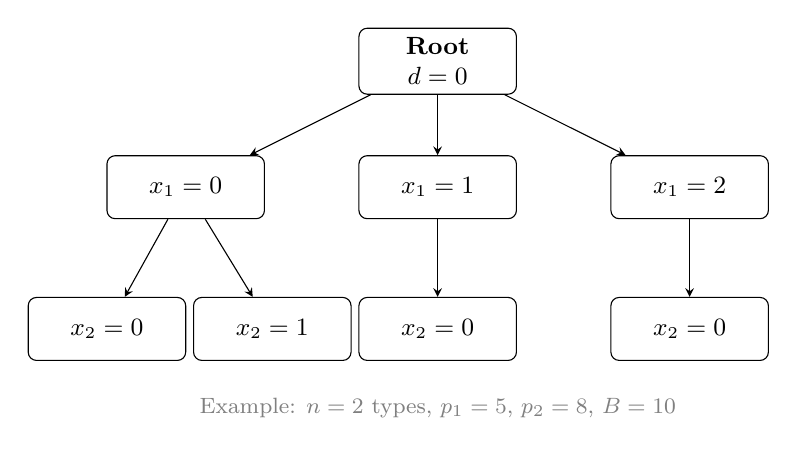
\begin{tikzpicture}[scale=1.0,
      nd/.style={draw,rectangle,rounded corners=3pt,
        font=\small,align=center,minimum width=2.0cm,minimum height=0.8cm},>=stealth]
    \node[nd](r)  at (0,4.2)    {\textbf{Root}\\$d=0$};
    \node[nd](n1) at (-3.2,2.6) {$x_1=0$};
    \node[nd](n2) at (0,2.6)    {$x_1=1$};
    \node[nd](n3) at (3.2,2.6)  {$x_1=2$};
    \node[nd](l1) at (-4.2,0.8) {$x_2=0$};
    \node[nd](l2) at (-2.1,0.8) {$x_2=1$};
    \node[nd](l3) at (0,0.8)    {$x_2=0$};
    \node[nd](l4) at (3.2,0.8)  {$x_2=0$};
    \draw[->](r)--(n1);\draw[->](r)--(n2);\draw[->](r)--(n3);
    \draw[->](n1)--(l1);\draw[->](n1)--(l2);
    \draw[->](n2)--(l3);\draw[->](n3)--(l4);
    \node[font=\footnotesize,gray] at (0,-0.2)
      {Example: $n=2$ types, $p_1=5$, $p_2=8$, $B=10$};
  \end{tikzpicture}
  \end{center}
  \smallskip
  Each \textbf{leaf} requires one follower (scheduling) solve.
  With large $n$ and $B$ the tree has billions of leaves $\Rightarrow$ intractable.
\end{frame}

% ===================================================================================
\section{Branch-and-Bound Algorithm}
% ===================================================================================

\begin{frame}[shrink=8]{Branch-and-Bound: Overview}
  \begin{block}{Node structure at depth $d$}
    \begin{itemize}
      \item \textbf{Fixed decisions:} $x_1,\ldots,x_d$\quad
            $\Brem = B - \sum_{i=1}^{d}p_ix_i$
      \item \textbf{Machine loads:} incremental LPT schedule for items $1,\ldots,d$
      \item \textbf{Children:} $x_{d+1}=0,1,\ldots,\lfloor\Brem/p_{d+1}\rfloor$
    \end{itemize}
  \end{block}
  \begin{columns}[T]
    \begin{column}{0.47\textwidth}
      \textbf{Three components:}
      \begin{enumerate}
        \item \textbf{Branching} — fix $x_{d}$
        \item \textbf{Bounding} — compute $\UB(d,\Brem)$
        \item \textbf{Pruning} — discard if $\UB\leq\Cinc$
      \end{enumerate}
    \end{column}
    \begin{column}{0.50\textwidth}
      \textbf{Design choices:}
      \begin{itemize}
        \item Depth-first $\to$ fast incumbent updates $\to$ aggressive pruning
        \item Incremental LPT: $O(m)$ per node
        \item DP precomputed: $O(1)$ bound lookups
      \end{itemize}
    \end{column}
  \end{columns}
\end{frame}

\begin{frame}[shrink=5]{The LPT Rule — Follower's Heuristic}
  \begin{columns}[T]
    \begin{column}{0.53\textwidth}
      \textbf{Longest Processing Time (LPT)} [Graham~1969]:
      \begin{itemize}
        \item Sort jobs by non-increasing duration
        \item Assign each to the \emph{least-loaded} machine
      \end{itemize}
      \textbf{Guarantee:}\quad $\Copt(x)\leq\Clpt(x)\leq\tfrac{4}{3}\Copt(x)$
      \begin{alertblock}{Incremental updates}
        Branching $d\to d{+}1$: append $x_{d+1}$ jobs of duration $d_{d+1}$.
        Reuse the existing sorted machine-load state — \textbf{no full recompute!}
      \end{alertblock}
    \end{column}
    \begin{column}{0.44\textwidth}
      \begin{block}{LPT algorithm}
        \footnotesize
        $L_1=\cdots=L_m\leftarrow 0$\\[0.15em]
        \textbf{for} each job $j$ (non-increasing order):\\
        \quad $k^*\leftarrow\arg\min_k L_k$\\
        \quad $L_{k^*}\leftarrow L_{k^*}+d_j$\\[0.15em]
        \textbf{return} $\Clpt=\max_k L_k$\\[0.2em]
        \normalsize Time: $O(J\log m)$
      \end{block}
      \textbf{Practice:} LPT is \emph{optimal} in $\approx84\%$ of our test instances.
    \end{column}
  \end{columns}
\end{frame}

\begin{frame}[shrink=5]{Pruning via Upper Bounds}
  At depth $d$ with remaining budget $\Brem$, we compute an \emph{upper bound}:
  \[\Copt(x_1,\ldots,x_n)\;\leq\;\UB(x_1,\ldots,x_d,\Brem)
    \quad\forall\text{ completions }x_{d+1},\ldots,x_n\]
  \textbf{Prune} whenever $\;\UB\leq\Cinc$.
  \[
    \UB = \underbrace{C_{\max}^{\mathrm{LPT},(d)}}_{\text{fixed items 1..}d}
         +\;\max_{\sum_{i>d}p_iy_i\leq\Brem}
           \underbrace{\Delta(y_{d+1},\ldots,y_n)}_{\text{extra makespan from remaining items}}
  \]
  \begin{columns}[T]
    \begin{column}{0.48\textwidth}
      \begin{block}{Ceiling bound}
        $\Delta = \sum_{i>d}d_i\lceil y_i/m\rceil$\\
        Single DP table, $O(1)$ lookup
      \end{block}
    \end{column}
    \begin{column}{0.48\textwidth}
      \begin{block}{Max-LPT bound}
        $\Delta = \Clpt(y_{d+1},\ldots,y_n)$\\
        DP table per depth, tighter bound
      \end{block}
    \end{column}
  \end{columns}
\end{frame}

% ===================================================================================
\section{The Ceiling Bound}
% ===================================================================================

\begin{frame}[shrink=5]{Ceiling Bound: Formulation}
  \begin{block}{Knapsack Scheduling Relaxation}
    \vspace{-0.3em}
    \[\UB = C_{\max}^{\mathrm{LPT},(d)}
      \;+\;
      \max_{y\geq 0}\;\sum_{i=d+1}^{n}d_i\!\left\lceil\frac{y_i}{m}\right\rceil
      \quad\text{s.t.}\;\sum_{i>d}p_iy_i\leq\Brem\]
    \vspace{-0.3em}
  \end{block}
  \textbf{Intuition:} $\lceil y_i/m\rceil$ jobs of type $i$ on $m$ equal machines raise makespan by
  $\lceil y_i/m\rceil\cdot d_i$ — always an \emph{overestimate}.
  \begin{block}{DP implementation — $O(1)$ lookup per node}
    \small Reduce to unbounded knapsack. For item type $i$:
    \begin{itemize}\small
      \item \textbf{Unit:} cost $p_i$, value $d_i$ (for $1,\ldots,m{-}1$ copies)
      \item \textbf{Block:} cost $m\cdot p_i$, value $d_i$ (for a batch of $m$)
    \end{itemize}
    Precompute in reverse item order $\Rightarrow$ any depth-$d$ query is a direct table read.
  \end{block}
\end{frame}

\begin{frame}[shrink=8]{Ceiling Bound: Validity Proof}
  \begin{block}{Theorem}
    For any feasible completion: $\Copt(x_1,\ldots,x_n)\leq\UB$
  \end{block}
  \textbf{Proof sketch:}
  \begin{enumerate}
    \item $\Copt(x)\leq\Clpt(x)$ (LPT over-schedules)
    \item After fixed items, current makespan $= C_{\max}^{\mathrm{LPT},(d)}$
    \item \emph{Assume} all machines filled to $C_{\max}^{\mathrm{LPT},(d)}$ — only inflates
    \item On $m$ equal-load machines, adding $y_i$ jobs of type $i$ raises makespan by
          $\lceil y_i/m\rceil\cdot d_i$
    \item Therefore $\Clpt(x)\leq C_{\max}^{\mathrm{LPT},(d)}+\sum_{i>d}\lceil x_i/m\rceil\cdot d_i$
    \item Maximising RHS over $\Brem$ gives $\UB\geq\Copt(x)$ \hfill$\square$
  \end{enumerate}
\end{frame}

% ===================================================================================
\section{The Max-LPT Bound}
% ===================================================================================

\begin{frame}[shrink=8]{The Max-LPT Problem}
  \begin{block}{Definition}
    Find $x\in\mathbb{Z}_+^n$ with $\sum_i p_ix_i\leq B$ that \textbf{maximises}~$\Clpt(x)$.
  \end{block}
  \begin{columns}[T]
    \begin{column}{0.54\textwidth}
      \textbf{Two roles:}
      \begin{enumerate}
        \item Solved once $\Rightarrow$ \textbf{strong initial incumbent} (with $\tfrac34$-approx.\ guarantee)
        \item Solved for remaining items at each node $\Rightarrow$ \textbf{tighter bound} than ceiling
      \end{enumerate}
      Respects actual LPT structure (not just $\lceil\cdot/m\rceil$).
    \end{column}
    \begin{column}{0.43\textwidth}
      \begin{alertblock}{Key result}
        Max-LPT solved \textbf{optimally} in $O(n\cdot B)$ via DP.
      \end{alertblock}
      \begin{block}{Trade-off}
        \small $n$ depth-specific DP tables vs.\ one ceiling table; recovered by better pruning.
      \end{block}
    \end{column}
  \end{columns}
\end{frame}

\begin{frame}[shrink=5]{Approximation Guarantee: Building Blocks}
  \begin{block}{Lemma (Properties of $\alpha$-approximation)}
    \vspace{-0.2em}
    \small Let \texttt{approx} be an $\alpha$-approx.\ for minimization ($\alpha\geq 1$), set $\beta:=1/\alpha$. Then for all $x$:
    \[\beta\cdot\mathrm{Opt}(x)\;\leq\;\beta\cdot\mathrm{approx}(x)\;\leq\;\mathrm{Opt}(x)\;\leq\;\mathrm{approx}(x)\]
    \vspace{-0.3em}
  \end{block}
  \begin{block}{Theorem (Bilevel Approx.\ [Weninger \& Fukasawa 2025])}
    \vspace{-0.2em}
    \small If $\beta\cdot\mathrm{Opt}(x)\leq\mathrm{approx}(x)\leq\mathrm{Opt}(x)\leq\mathrm{approx}(x)$ for all $x$ and $\hat x\in\arg\max_x\,\mathrm{approx}(x)$, then:
    \[\beta\cdot\mathrm{Opt}_{\text{bilevel}}\;\leq\;\mathrm{Opt}(\hat x)\;\leq\;\mathrm{Opt}_{\text{bilevel}}\]
    \vspace{-0.3em}
  \end{block}
  \textbf{Our setting:} LPT is a $\tfrac{4}{3}$-approx.\ for $P||\Cmax$ $\Rightarrow$ $\beta=\tfrac{3}{4}$. Max-LPT maximises $\Clpt$ $\Rightarrow$ apply Theorem directly.
\end{frame}

\begin{frame}[shrink=5]{The $\frac{3}{4}$-Approximation Guarantee}
  \begin{block}{Theorem}
    Let $\hat x$ be the Max-LPT solution and $x^*$ the bilevel-optimal solution. Then:
    \[\tfrac{3}{4}\,\Copt(x^*)\;\leq\;\Copt(\hat x)\;\leq\;\Copt(x^*)\]
  \end{block}
  \textbf{Proof} (using the two building blocks):
  \begin{enumerate}\small
    \item \textbf{Lemma} ($\alpha=\tfrac{4}{3}$, $\beta=\tfrac{3}{4}$): for all $x$,\quad $\tfrac34\,\Copt(x)\leq\tfrac34\,\Clpt(x)\leq\Copt(x)\leq\Clpt(x)$
    \item $\hat x$ maximises $\Clpt$, so $\;\Clpt(x^*)\leq\Clpt(\hat x)$
    \item \textbf{Theorem [WF25]:}\quad $\tfrac{3}{4}\cdot\mathrm{Opt}_{\text{bilevel}}\leq\Copt(\hat x)\leq\mathrm{Opt}_{\text{bilevel}}$
    \item \textbf{Full chain:}\quad $\tfrac34\,\Copt(x^*)\leq\tfrac34\,\Clpt(x^*)\leq\tfrac34\,\Clpt(\hat x)\leq\Copt(\hat x)\leq\Copt(x^*)$ \hfill$\square$
  \end{enumerate}
  \begin{alertblock}{Practical implication}
    The Max-LPT incumbent is \textbf{guaranteed $\leq 25\%$ suboptimal}.
    In practice the gap is virtually always zero (LPT is often optimal).
  \end{alertblock}
\end{frame}

\begin{frame}[shrink=40]{Max-LPT Algorithm: Per-Machine Budget \& Properties}
    \begin{block}{Structural observation}
    In any LPT schedule, the \textbf{job that finishes last} $I$ was put on the \textbf{least-loaded machine at the time of scheduling}:
    \[\Clpt = C_{\max}^{(m)} + d_I\]
    Makespan is determined by the \emph{minimum machine load} just before $I$ plus its duration $d_I$.
  \end{block}
  For a fixed candidate last job $J$, we want to maximise $C_{\max}^{(m)}$ for items $1,\ldots,J$.
  \begin{block}{Two key properties of the optimal preceding schedule}
    \begin{itemize}
      \item \textbf{Property 1} (highest per-machine budget):\\
            $B^* := \lfloor B/m \rfloor$ is the largest budget assignable equally to each machine.\\
            No redistribution can give the least-loaded machine more than $B^*$.
      \item \textbf{Property 2} (best items for $B^*$):\\
            Given budget $B^*$, the optimal item combination from types $\leq J$ is the unbounded knapsack optimum.
    \end{itemize}
    If both hold, no schedule achieves a larger $C_{\max}^{(m)}$: buy $m$ copies of every DP-optimal item and run LPT.
  \end{block}
  \begin{block}{Budget adjustment when $\hat{B} := B - mB^* < p_J$}
    \small Remainder $\hat{B}$ is too small to pay for one copy of $J$.
    Reduce $B^*$ by 1 (uniformly across machines) until $\hat{B} \geq p_J$.
    Property 1 holds for the reduced $B^*$; re-query $\mathrm{DP}(J,B^*)$.
    If $B^*$ reaches~0 before $\hat{B} \geq p_J$, skip $J$ (infeasible).
  \end{block}
\end{frame}

\begin{frame}[shrink=40]{Max-LPT Algorithm: Correctness \& Complexity}
  \begin{block}{Algorithm (pseudocode)}
    \small
    Precompute DP table (unbounded knapsack, items $1\ldots n$, budgets $0\ldots B$).\\[0.2em]
    $z^*\leftarrow 0$\hfill\emph{// best candidate so far}\\
    \textbf{for} each type $J\in\{1,\ldots,n\}$:\\
    \qquad $B^*\leftarrow\lfloor B/m\rfloor$\\
    \qquad \textbf{while} $(B-mB^*)<p_J$ \textbf{and} $B^*>0$:\; $B^*\leftarrow B^*-1$\\
    \qquad \textbf{if} $(B-mB^*)<p_J$: skip $J$\hfill\emph{// infeasible}\\
    \qquad $z_J\leftarrow\mathrm{DP}(J,B^*)+d_J$;\; $z^*\leftarrow\max(z^*,z_J)$\\
    \textbf{return} $z^*$
  \end{block}
  \begin{columns}[T]
    \begin{column}{0.53\textwidth}
      \begin{block}{Correctness}
        \small
        Any optimal solution has a last job $I$ matching Case 1 or 2.\\[0.2em]
        For that $I$, Properties 1 \& 2 identify the optimal preceding schedule via $\mathrm{DP}(I,B^*)$.\\[0.2em]
        Taking $\max_J z_J$ over all candidates covers it.\hfill$\square$
      \end{block}
    \end{column}
    \begin{column}{0.44\textwidth}
      \begin{alertblock}{Complexity: $O(n\cdot B)$}
        \small
        DP table precomputed in $O(n\cdot B)$.\\[0.2em]
        Per candidate $J$: $O(1)$ lookup + $O(B^*/m)$ adjustment.\\[0.2em]
        $n$ candidates $\Rightarrow O(n\cdot B)$ total.
      \end{alertblock}
    \end{column}
  \end{columns}
\end{frame}

% ===================================================================================
\section{Early Optimality Detection}
% ===================================================================================

\begin{frame}[shrink=5]{Early Optimality Detection}
  \begin{block}{Key inequality}
    For all $x$: $\Copt(x)\leq\Clpt(x)$ (LPT only overestimates)
  \end{block}
  Let $\hat x\in\arg\max_x\Clpt(x)$. If $\Clpt(\hat x)=\Copt(\hat x)$, then for \emph{any} feasible $x$:
  \[\Copt(\hat x)=\Clpt(\hat x)\geq\Clpt(x)\geq\Copt(x)\]
  $\Rightarrow$ $\hat x$ is the \textbf{global bilevel optimum} - no B\&B tree needed!
  \begin{alertblock}{Impact}
    \begin{itemize}
      \item $\Copt(\hat x)$ is computed anyway to initialise the incumbent
      \item This check costs \textbf{nothing extra}
      \item Triggered in $\approx\mathbf{84.6\%}$ of our test instances $\Rightarrow$ solved at root
    \end{itemize}
  \end{alertblock}
\end{frame}

\begin{frame}[shrink=5]{Complete Algorithm}
  \begin{columns}[T]
    \begin{column}{0.53\textwidth}
      \small
      \begin{enumerate}
        \item Solve Max-LPT $\to\hat x$;\quad compute $\Clpt(\hat x)$, $\Copt(\hat x)$
        \item \textbf{If} $\Clpt(\hat x)=\Copt(\hat x)$: \textbf{return} $\hat x$
        \item $\Cinc\leftarrow\Copt(\hat x)$;\quad push root to stack $Q$
        \item \textbf{While} $Q\neq\emptyset$:
        \begin{itemize}\small
          \item Remove node $(d,x_1,\ldots,x_d,\Brem)$
          \item If $d=n$: solve follower; update $\Cinc$
          \item Else: compute $\UB(d,\Brem)$
          \item If $\UB\leq\Cinc$: \textbf{prune}
          \item Else: push children (depth-first)
        \end{itemize}
        \item Return incumbent
      \end{enumerate}
      \smallskip
      {\footnotesize Inspired by [Weninger \& Fukasawa 2025].}
    \end{column}
    \begin{column}{0.44\textwidth}
      \begin{block}{Leaf optimisation}
        \small At depth $n{-}1$: only the child spending \emph{maximum} remaining budget matters.
        All others produce a smaller or equal $\Copt$.
      \end{block}
      \begin{block}{Follower solver}
        \small Gurobi 12.0.3 [Gurobi Optimization 2024] solves the MIP formulation of $P||\Cmax$ at leaves.
      \end{block}
    \end{column}
  \end{columns}
\end{frame}

% ===================================================================================
\section{Computational Experiments}
% ===================================================================================

\begin{frame}[shrink=5]{Experimental Setup}
  \begin{columns}[T]
    \begin{column}{0.50\textwidth}
      \textbf{Hardware \& software:}
      \begin{itemize}
        \item AMD Ryzen 5 9600X, 32\,GB RAM
        \item Python 3.11, Gurobi 12.0.3
        \item Single-threaded runs
      \end{itemize}
      \textbf{PatternTestSet:} 140 instances\\
      7 structural patterns:\\
      \footnotesize Uniform Ratios, High Variance, Increasing, Random Moderate,
      Extreme, Strong Correlation, Subset Sum\\
      \normalsize 6--12 types, 3--8 machines, budget 15--50
    \end{column}
    \begin{column}{0.47\textwidth}
      \begin{block}{Correctness: vs.\ enumeration}
        \begin{itemize}
          \item 140 instances: \textbf{0 discrepancies}
          \item Enumeration timed out on 15/140
          \item B\&B solved all 140 in ms
        \end{itemize}
      \end{block}
      \begin{alertblock}{Speed-up}
        Up to $\mathbf{10^6\times}$ faster\\than complete enumeration
      \end{alertblock}
    \end{column}
  \end{columns}
\end{frame}

\begin{frame}[shrink=8]{Grid Sensitivity Analysis}
  \textbf{Grid:} $6{\times}6$ (types $\times$ machines), 3 budget multipliers, 5 seeds $=540$ instances; 1\,h limit.\\[0.15em]
  \footnotesize\textbf{Types:} 4, 8, 12, 16, 20, 24\quad\textbullet\quad\textbf{Machines:} 2, 4, 6, 8, 10, 12\quad\textbullet\quad\textbf{Multipliers:} 1.3, 2.5, 5.0\normalsize

  \begin{center}\small
  \begin{tabular}{lrrrr}
    \toprule
    Budget $\times$ & Root Opt. & Completed & Timeout & Leaf T/O\\
    \midrule
    $1.3\times$ & 154\,/\,154 & 22\,/\,26 & 2\,/\,0 & 2\,/\,0\\
    $2.5\times$ & 150\,/\,150 & 19\,/\,22 & 3\,/\,0 & 8\,/\,8\\
    $5.0\times$ & 153\,/\,153 & 20\,/\,23 & 4\,/\,1 & 3\,/\,3\\
    \bottomrule
  \end{tabular}\\[0.2em]
  \footnotesize Ceil\,/\,MaxLPT
  \end{center}

  \begin{columns}[T]
    \begin{column}{0.48\textwidth}
      \begin{alertblock}{Main finding}
        $\mathbf{84.6\%}$ of instances solved at root —
        no B\&B tree needed
      \end{alertblock}
    \end{column}
    \begin{column}{0.48\textwidth}
      \begin{block}{MaxLPT advantage}
        More completions and fewer timeouts in every setting
      \end{block}
    \end{column}
  \end{columns}
\end{frame}

\begin{frame}[shrink=5]{Ceiling vs.\ MaxLPT: Hard Instances}
  61 non-root-optimal instances where both bounds completed within 1\,h:
  \begin{columns}[T]
    \begin{column}{0.49\textwidth}
      \textbf{Runtime (Ceiling $-$ MaxLPT):}
      \begin{itemize}
        \item Mean: $+71$\,s (ceiling slower)
        \item Median: $+0.4$\,s
        \item Max: $+1{,}057$\,s
        \item MaxLPT faster: \textbf{41 of 61 cases}
      \end{itemize}
    \end{column}
    \begin{column}{0.49\textwidth}
      \textbf{Nodes (Ceiling $-$ MaxLPT):}
      \begin{itemize}
        \item Mean: $+4.8$M nodes
        \item Median: $+69$K
        \item Max: $+54.5$M
        \item MaxLPT always fewer nodes
      \end{itemize}
    \end{column}
  \end{columns}
  \begin{block}{Interpretation}
    \small MaxLPT prunes more aggressively on hard instances.
    Precomputing $n$ DP tables is fully justified by the reduced node count.
    Ceiling is marginally faster for trivial (root-optimal) cases.
  \end{block}
\end{frame}

\begin{frame}[shrink=5]{Comparison with MibS}
  \textbf{MibS}: general-purpose bilevel MILP solver [Tahernejad et al.\ 2020]\\
  \textbf{Subset:} $m\in\{4,8,12\}$, $j\in\{4,8,16,20\}$, 3 multipliers, 5 seeds $=180$ instances

  \begin{center}\small
  \begin{tabular}{crrrr}
    \toprule
    $m\;\backslash\; j$ & 4 & 8 & 16 & 20\\
    \midrule
    4  & 15/15 & 8/15 & 2/15 & 1/15\\
    8  & 5/15  & 0/15 & 0/15 & 1/15\\
    12 & 2/15  & 0/15 & 0/15 & 0/15\\
    \bottomrule
  \end{tabular}\\[0.2em]
  {\footnotesize MibS completions (of 15) per cell. MaxLPT B\&B: \textbf{179/180}.}
  \end{center}

  \begin{alertblock}{Speed-up over MibS (1\,h limit)}
    \small Ceiling: mean $+2{,}876.6$\,s, median $+3{,}599.9$\,s\quad
    MaxLPT: mean $+2{,}959.6$\,s, median $+3{,}599.5$\,s\\
    Problems solved by our algorithm in milliseconds require \textbf{over an hour} for MibS.
  \end{alertblock}
\end{frame}

% ===================================================================================
\section{Conclusion}
% ===================================================================================

\begin{frame}[shrink=5]{Summary \& Conclusions}
  \begin{columns}[T]
    \begin{column}{0.55\textwidth}
      \textbf{Contributions:}
      \begin{enumerate}
        \item Formal bilevel knapsack-scheduling model
        \item Ceiling bound with precomputed $O(1)$ DP, solvable in $O(n\cdot B)$
        \item Max-LPT solved optimally in $O(n\cdot B)$
        \item $\tfrac34$-approximation guarantee (theory)
        \item Early optimality detection ($84.6\%$ solve at root)
        \item Comprehensive computational study
      \end{enumerate}
      \smallskip
      Outperforms MibS by \textbf{orders of magnitude}.
    \end{column}
    \begin{column}{0.42\textwidth}
      \begin{alertblock}{Limitations}
        \small
        \begin{itemize}
          \item No characterisation of easy instances
          \item Identical machines only
        \end{itemize}
      \end{alertblock}
      \begin{block}{Future work}
        \small
        \begin{itemize}
          \item Related/unrelated machines
          \item Stochastic processing times
          \item Characterise root-optimal instances
        \end{itemize}
      \end{block}
    \end{column}
  \end{columns}
\end{frame}

\begin{frame}[plain]
  \begin{center}
    \vspace{3em}
    {\huge\bfseries Thank you!}\\[0.8em]
    {\Large Questions?}\\[1.6em]
    \rule{8cm}{0.4pt}\\[0.4em]
    {\small Ole Damke \;\textbullet\; \texttt{o.damke@tu-braunschweig.de}\\[0.2em]
           Institut für Mathematische Optimierung \;\textbullet\; TU Braunschweig}
  \end{center}
\end{frame}

% ===================================================================================
\appendix

\begin{frame}[allowframebreaks]{References}
  \footnotesize
  \begin{thebibliography}{9}
    \bibitem{frangioni1995}
      A.\,Frangioni. On a new class of bilevel programming problems and its use
      for reformulating mixed integer problems.
      \textit{Eur.~J.~Oper.~Res.}, 82(3):615--646, 1995.
    \bibitem{graham1969}
      R.\,L.\,Graham. Bounds on Multiprocessor Timing Anomalies.
      \textit{SIAM J.\ Appl.\ Math.}, 17(2):416--429, 1969.
    \bibitem{weninger2025}
      N.\,Weninger, R.\,Fukasawa. A fast combinatorial algorithm for the bilevel knapsack problem.
      \textit{Math.\ Program.}, 210(1):847--879, 2025.
    \bibitem{tahernejad2020}
      S.\,Tahernejad, T.\,K.\,Ralphs, S.\,T.\,DeNegre. A branch-and-cut algorithm for mixed
      integer bilevel linear optimisation.
      \textit{Math.\ Program.\ Comput.}, 12(4):529--568, 2020.
    \bibitem{kleinert2021}
      T.\,Kleinert et al. A survey on MIP techniques in bilevel optimisation.
      \textit{EURO J.\ Comput.\ Optim.}, 9:100007, 2021.
    \bibitem{dempe2020}
      S.\,Dempe, A.\,Zemkoho. \textit{Bilevel Optimization}, vol.\,161. Springer, 2020.
    \bibitem{gurobi2024}
      Gurobi Optimization, LLC. \textit{Gurobi Optimizer Reference Manual}. Version 12.0, 2024.
      \url{https://www.gurobi.com}
  \end{thebibliography}
\end{frame}

\end{document}
